\documentclass[twoside]{book}

% Packages required by doxygen
\usepackage{fixltx2e}
\usepackage{calc}
\usepackage{doxygen}
\usepackage[export]{adjustbox} % also loads graphicx
\usepackage{graphicx}
\usepackage[utf8]{inputenc}
\usepackage{makeidx}
\usepackage{multicol}
\usepackage{multirow}
\PassOptionsToPackage{warn}{textcomp}
\usepackage{textcomp}
\usepackage[nointegrals]{wasysym}
\usepackage[table]{xcolor}

% Font selection
\usepackage[T1]{fontenc}
\usepackage[scaled=.90]{helvet}
\usepackage{courier}
\usepackage{amssymb}
\usepackage{sectsty}
\renewcommand{\familydefault}{\sfdefault}
\allsectionsfont{%
  \fontseries{bc}\selectfont%
  \color{darkgray}%
}
\renewcommand{\DoxyLabelFont}{%
  \fontseries{bc}\selectfont%
  \color{darkgray}%
}
\newcommand{\+}{\discretionary{\mbox{\scriptsize$\hookleftarrow$}}{}{}}

% Page & text layout
\usepackage{geometry}
\geometry{%
  a4paper,%
  top=2.5cm,%
  bottom=2.5cm,%
  left=2.5cm,%
  right=2.5cm%
}
\tolerance=750
\hfuzz=15pt
\hbadness=750
\setlength{\emergencystretch}{15pt}
\setlength{\parindent}{0cm}
\setlength{\parskip}{3ex plus 2ex minus 2ex}
\makeatletter
\renewcommand{\paragraph}{%
  \@startsection{paragraph}{4}{0ex}{-1.0ex}{1.0ex}{%
    \normalfont\normalsize\bfseries\SS@parafont%
  }%
}
\renewcommand{\subparagraph}{%
  \@startsection{subparagraph}{5}{0ex}{-1.0ex}{1.0ex}{%
    \normalfont\normalsize\bfseries\SS@subparafont%
  }%
}
\makeatother

% Headers & footers
\usepackage{fancyhdr}
\pagestyle{fancyplain}
\fancyhead[LE]{\fancyplain{}{\bfseries\thepage}}
\fancyhead[CE]{\fancyplain{}{}}
\fancyhead[RE]{\fancyplain{}{\bfseries\leftmark}}
\fancyhead[LO]{\fancyplain{}{\bfseries\rightmark}}
\fancyhead[CO]{\fancyplain{}{}}
\fancyhead[RO]{\fancyplain{}{\bfseries\thepage}}
\fancyfoot[LE]{\fancyplain{}{}}
\fancyfoot[CE]{\fancyplain{}{}}
\fancyfoot[RE]{\fancyplain{}{\bfseries\scriptsize Generated by Doxygen }}
\fancyfoot[LO]{\fancyplain{}{\bfseries\scriptsize Generated by Doxygen }}
\fancyfoot[CO]{\fancyplain{}{}}
\fancyfoot[RO]{\fancyplain{}{}}
\renewcommand{\footrulewidth}{0.4pt}
\renewcommand{\chaptermark}[1]{%
  \markboth{#1}{}%
}
\renewcommand{\sectionmark}[1]{%
  \markright{\thesection\ #1}%
}

% Indices & bibliography
\usepackage{natbib}
\usepackage[titles]{tocloft}
\setcounter{tocdepth}{3}
\setcounter{secnumdepth}{5}
\makeindex

% Hyperlinks (required, but should be loaded last)
\usepackage{ifpdf}
\ifpdf
  \usepackage[pdftex,pagebackref=true]{hyperref}
\else
  \usepackage[ps2pdf,pagebackref=true]{hyperref}
\fi
\hypersetup{%
  colorlinks=true,%
  linkcolor=blue,%
  citecolor=blue,%
  unicode%
}

% Custom commands
\newcommand{\clearemptydoublepage}{%
  \newpage{\pagestyle{empty}\cleardoublepage}%
}

\usepackage{caption}
\captionsetup{labelsep=space,justification=centering,font={bf},singlelinecheck=off,skip=4pt,position=top}

%===== C O N T E N T S =====

\begin{document}

% Titlepage & ToC
\hypersetup{pageanchor=false,
             bookmarksnumbered=true,
             pdfencoding=unicode
            }
\pagenumbering{alph}
\begin{titlepage}
\vspace*{7cm}
\begin{center}%
{\Large My Project }\\
\vspace*{1cm}
{\large Generated by Doxygen 1.8.12}\\
\end{center}
\end{titlepage}
\clearemptydoublepage
\pagenumbering{roman}
\tableofcontents
\clearemptydoublepage
\pagenumbering{arabic}
\hypersetup{pageanchor=true}

%--- Begin generated contents ---
\chapter{Hierarchical Index}
\section{Class Hierarchy}
This inheritance list is sorted roughly, but not completely, alphabetically\+:\begin{DoxyCompactList}
\item \contentsline{section}{crew}{\pageref{classcrew}}{}
\item Q\+Dialog\begin{DoxyCompactList}
\item \contentsline{section}{credit}{\pageref{classcredit}}{}
\item \contentsline{section}{edit}{\pageref{classedit}}{}
\item \contentsline{section}{Edit\+Aud}{\pageref{class_edit_aud}}{}
\end{DoxyCompactList}
\item Q\+Main\+Window\begin{DoxyCompactList}
\item \contentsline{section}{Login}{\pageref{class_login}}{}
\item \contentsline{section}{Login}{\pageref{class_login}}{}
\end{DoxyCompactList}
\item Q\+Widget\begin{DoxyCompactList}
\item \contentsline{section}{Data\+Base}{\pageref{class_data_base}}{}
\item \contentsline{section}{showtata}{\pageref{classshowtata}}{}
\end{DoxyCompactList}
\item \contentsline{section}{stage}{\pageref{classstage}}{}
\end{DoxyCompactList}

\chapter{Class Index}
\section{Class List}
Here are the classes, structs, unions and interfaces with brief descriptions\+:\begin{DoxyCompactList}
\item\contentsline{section}{\hyperlink{class_data_base}{Data\+Base} }{\pageref{class_data_base}}{}
\item\contentsline{section}{\hyperlink{class_login}{Login} }{\pageref{class_login}}{}
\item\contentsline{section}{\hyperlink{classshowtata}{showtata} }{\pageref{classshowtata}}{}
\item\contentsline{section}{\hyperlink{class_s_q_l_c_o_n}{S\+Q\+L\+C\+ON} }{\pageref{class_s_q_l_c_o_n}}{}
\item\contentsline{section}{\hyperlink{classsql_settings}{sql\+Settings} }{\pageref{classsql_settings}}{}
\end{DoxyCompactList}

\chapter{Class Documentation}
\hypertarget{class_data_base}{}\section{Data\+Base Class Reference}
\label{class_data_base}\index{Data\+Base@{Data\+Base}}
Inheritance diagram for Data\+Base\+:\begin{figure}[H]
\begin{center}
\leavevmode
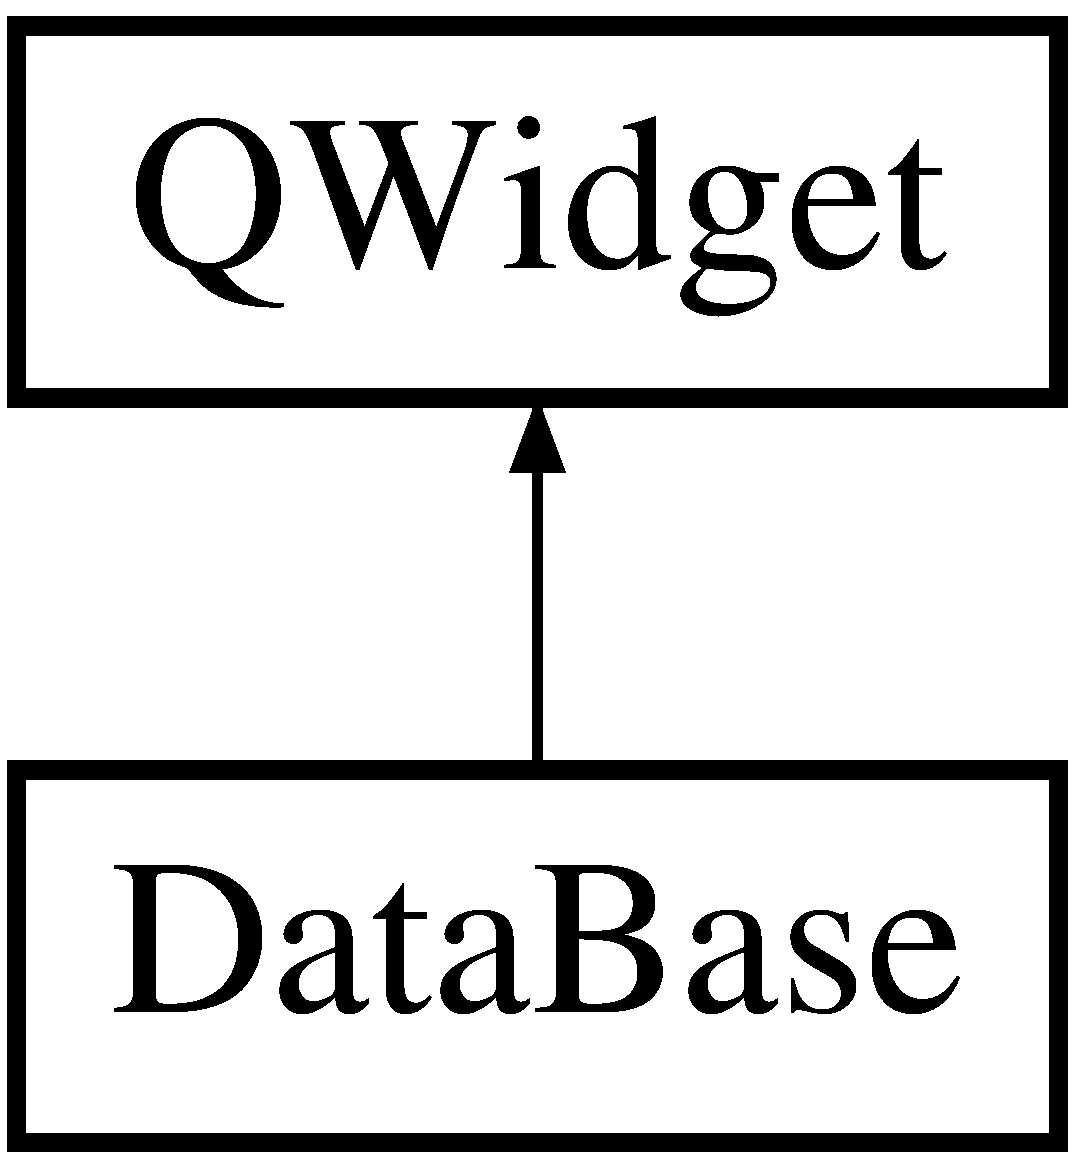
\includegraphics[height=2.000000cm]{class_data_base}
\end{center}
\end{figure}
\subsection*{Public Member Functions}
\begin{DoxyCompactItemize}
\item 
\hypertarget{class_data_base_a54fde8aa4dfdc9ce978f2985877caf6c}{}\label{class_data_base_a54fde8aa4dfdc9ce978f2985877caf6c} 
{\bfseries Data\+Base} (Q\+Widget $\ast$parent=0)
\end{DoxyCompactItemize}


The documentation for this class was generated from the following files\+:\begin{DoxyCompactItemize}
\item 
database.\+h\item 
database.\+cpp\end{DoxyCompactItemize}

\hypertarget{class_login}{}\section{Login Class Reference}
\label{class_login}\index{Login@{Login}}
Inheritance diagram for Login\+:\begin{figure}[H]
\begin{center}
\leavevmode
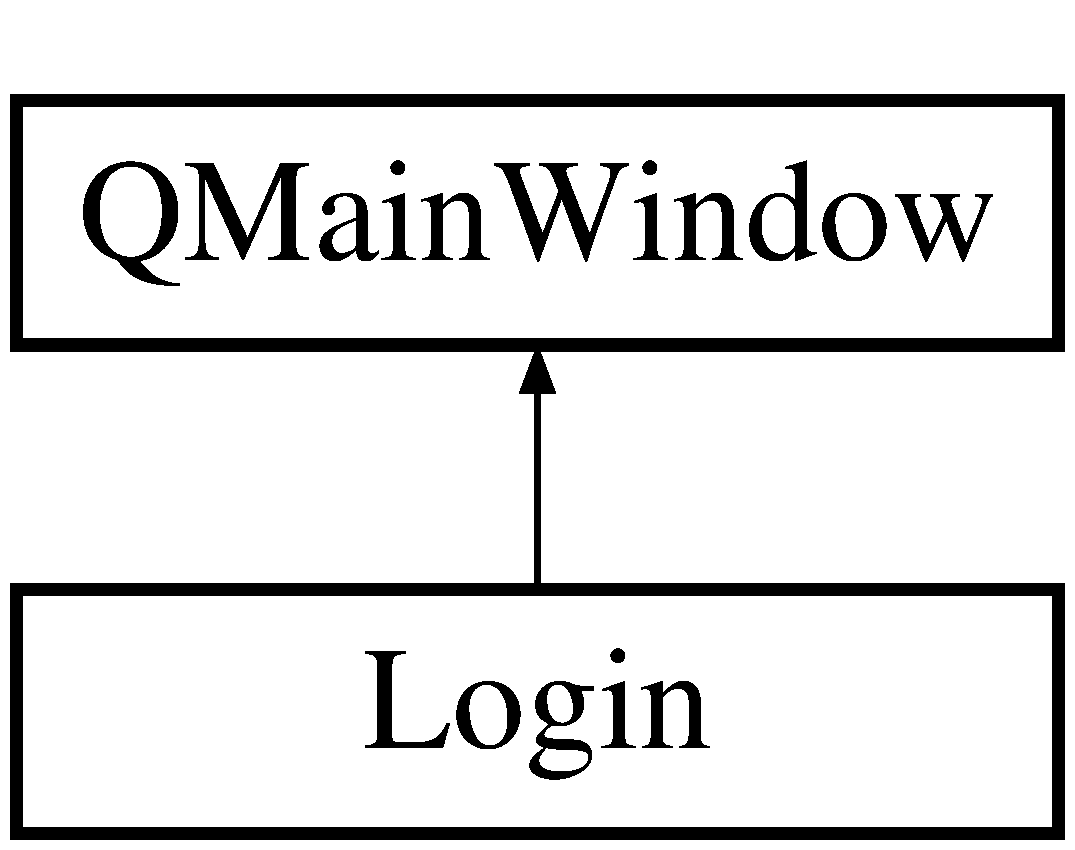
\includegraphics[height=2.000000cm]{class_login}
\end{center}
\end{figure}
\subsection*{Public Member Functions}
\begin{DoxyCompactItemize}
\item 
\hypertarget{class_login_a021ebcfd29b2a30e3f5c5bbb36589381}{}\label{class_login_a021ebcfd29b2a30e3f5c5bbb36589381} 
{\bfseries Login} (Q\+Widget $\ast$parent=0)
\item 
\hypertarget{class_login_ad6a6b037140e8823d1b290cbcfeb2087}{}\label{class_login_ad6a6b037140e8823d1b290cbcfeb2087} 
void {\bfseries loadsettings} ()
\item 
\hypertarget{class_login_aac2415f9743fe56e19c5488fabf4aaba}{}\label{class_login_aac2415f9743fe56e19c5488fabf4aaba} 
void {\bfseries savesettings} ()
\item 
\hypertarget{class_login_a5060f9bd0638df8820f80ecde59c801f}{}\label{class_login_a5060f9bd0638df8820f80ecde59c801f} 
void {\bfseries set\+Begin\+Seting} ()
\item 
\hypertarget{class_login_a021ebcfd29b2a30e3f5c5bbb36589381}{}\label{class_login_a021ebcfd29b2a30e3f5c5bbb36589381} 
{\bfseries Login} (Q\+Widget $\ast$parent=0)
\item 
\hypertarget{class_login_ad6a6b037140e8823d1b290cbcfeb2087}{}\label{class_login_ad6a6b037140e8823d1b290cbcfeb2087} 
void {\bfseries loadsettings} ()
\item 
\hypertarget{class_login_aac2415f9743fe56e19c5488fabf4aaba}{}\label{class_login_aac2415f9743fe56e19c5488fabf4aaba} 
void {\bfseries savesettings} ()
\item 
\hypertarget{class_login_a5060f9bd0638df8820f80ecde59c801f}{}\label{class_login_a5060f9bd0638df8820f80ecde59c801f} 
void {\bfseries set\+Begin\+Seting} ()
\end{DoxyCompactItemize}
\subsection*{Public Attributes}
\begin{DoxyCompactItemize}
\item 
\hypertarget{class_login_aeab33b7e36bd3e55c6a957290a74e221}{}\label{class_login_aeab33b7e36bd3e55c6a957290a74e221} 
Q\+Action $\ast$ {\bfseries Setting}
\item 
\hypertarget{class_login_a8c0727b99b15f38a77ab946fa3239801}{}\label{class_login_a8c0727b99b15f38a77ab946fa3239801} 
Q\+Message\+Box $\ast$ {\bfseries mes1}
\item 
\hypertarget{class_login_af88cd8be1e64096bdca27d016e60e719}{}\label{class_login_af88cd8be1e64096bdca27d016e60e719} 
\hyperlink{classshowtata}{showtata} $\ast$ {\bfseries dod}
\item 
\hypertarget{class_login_a7033035a95e1f9ab15f9ed9c2da9ceeb}{}\label{class_login_a7033035a95e1f9ab15f9ed9c2da9ceeb} 
\hyperlink{class_login}{Login} $\ast$ {\bfseries main}
\end{DoxyCompactItemize}


The documentation for this class was generated from the following files\+:\begin{DoxyCompactItemize}
\item 
login.\+h\item 
login\+\_\+copy.\+h\item 
login.\+cpp\end{DoxyCompactItemize}

\hypertarget{classshowtata}{}\section{showtata Class Reference}
\label{classshowtata}\index{showtata@{showtata}}
Inheritance diagram for showtata\+:\begin{figure}[H]
\begin{center}
\leavevmode
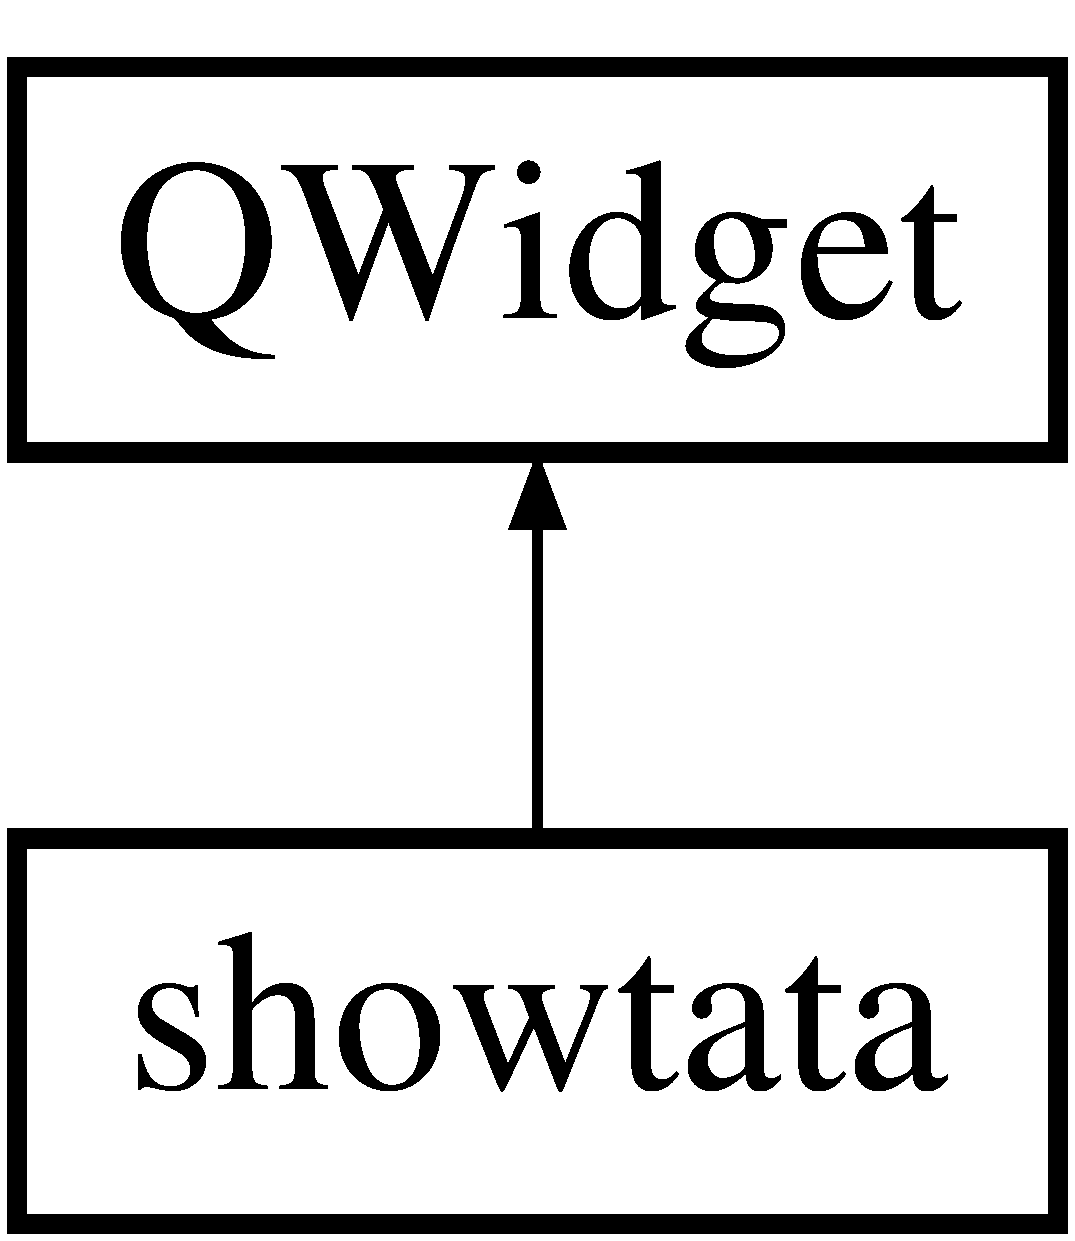
\includegraphics[height=2.000000cm]{classshowtata}
\end{center}
\end{figure}
\subsection*{Signals}
\begin{DoxyCompactItemize}
\item 
\hypertarget{classshowtata_af7c54c814de835f906e841b9ecaa6643}{}\label{classshowtata_af7c54c814de835f906e841b9ecaa6643} 
bool {\bfseries closed} ()
\end{DoxyCompactItemize}
\subsection*{Public Member Functions}
\begin{DoxyCompactItemize}
\item 
\hypertarget{classshowtata_a8b9382b64c639b083122cf4a5cee975d}{}\label{classshowtata_a8b9382b64c639b083122cf4a5cee975d} 
{\bfseries showtata} (Q\+Widget $\ast$parent=0)
\end{DoxyCompactItemize}
\subsection*{Public Attributes}
\begin{DoxyCompactItemize}
\item 
\hypertarget{classshowtata_a221cbd798a46ba1c75062e358bc17ad2}{}\label{classshowtata_a221cbd798a46ba1c75062e358bc17ad2} 
\hyperlink{classedit}{edit} $\ast$ {\bfseries edemp}
\item 
\hypertarget{classshowtata_ace79d422d191a7cf665c216495250a62}{}\label{classshowtata_ace79d422d191a7cf665c216495250a62} 
\hyperlink{class_edit_aud}{Edit\+Aud} $\ast$ {\bfseries edaud}
\end{DoxyCompactItemize}


The documentation for this class was generated from the following files\+:\begin{DoxyCompactItemize}
\item 
showtata.\+h\item 
showtata.\+cpp\end{DoxyCompactItemize}

\hypertarget{class_s_q_l_c_o_n}{}\section{S\+Q\+L\+C\+ON Class Reference}
\label{class_s_q_l_c_o_n}\index{S\+Q\+L\+C\+ON@{S\+Q\+L\+C\+ON}}
\subsection*{Public Member Functions}
\begin{DoxyCompactItemize}
\item 
\hypertarget{class_s_q_l_c_o_n_a4b5fe8f86c8f7e5ef789ae83d77783b3}{}\label{class_s_q_l_c_o_n_a4b5fe8f86c8f7e5ef789ae83d77783b3} 
void {\bfseries connetct} (Q\+Object $\ast$parent)
\item 
\hypertarget{class_s_q_l_c_o_n_a8bf29da8885cda8568217d238a3f9a70}{}\label{class_s_q_l_c_o_n_a8bf29da8885cda8568217d238a3f9a70} 
void {\bfseries load\+Settings} ()
\item 
\hypertarget{class_s_q_l_c_o_n_a2189744edaf1ee3e4cf29e78cf3d412a}{}\label{class_s_q_l_c_o_n_a2189744edaf1ee3e4cf29e78cf3d412a} 
void {\bfseries save\+Settings} ()
\item 
\hypertarget{class_s_q_l_c_o_n_ac4aca7afd1ec62ba3ebf9b5701bf7d2a}{}\label{class_s_q_l_c_o_n_ac4aca7afd1ec62ba3ebf9b5701bf7d2a} 
int {\bfseries get\+Port} () const
\item 
\hypertarget{class_s_q_l_c_o_n_a33d33265a3cd24202c0783b77b4f9360}{}\label{class_s_q_l_c_o_n_a33d33265a3cd24202c0783b77b4f9360} 
void {\bfseries set\+Port} (const int \&value)
\item 
\hypertarget{class_s_q_l_c_o_n_a54ecc284e59e35653280b8c091702255}{}\label{class_s_q_l_c_o_n_a54ecc284e59e35653280b8c091702255} 
Q\+String {\bfseries get\+Pass} () const
\item 
\hypertarget{class_s_q_l_c_o_n_a381507ec32fcb1006d0d141ba3510e15}{}\label{class_s_q_l_c_o_n_a381507ec32fcb1006d0d141ba3510e15} 
void {\bfseries set\+Pass} (const Q\+String \&value)
\item 
\hypertarget{class_s_q_l_c_o_n_ac03190b87c99cedee7ba762a78ab1308}{}\label{class_s_q_l_c_o_n_ac03190b87c99cedee7ba762a78ab1308} 
Q\+String {\bfseries get\+Login} () const
\item 
\hypertarget{class_s_q_l_c_o_n_a36a5c1a719e6b67be73ed075d96084a2}{}\label{class_s_q_l_c_o_n_a36a5c1a719e6b67be73ed075d96084a2} 
void {\bfseries set\+Login} (const Q\+String \&value)
\item 
\hypertarget{class_s_q_l_c_o_n_a9490fdf5df564cc032dec7424eb619d8}{}\label{class_s_q_l_c_o_n_a9490fdf5df564cc032dec7424eb619d8} 
Q\+String {\bfseries get\+Ip} () const
\item 
\hypertarget{class_s_q_l_c_o_n_a550d016acbe567d39b305e2a7fb8f28b}{}\label{class_s_q_l_c_o_n_a550d016acbe567d39b305e2a7fb8f28b} 
void {\bfseries set\+Ip} (const Q\+String \&value)
\item 
\hypertarget{class_s_q_l_c_o_n_ac6f8507d63e35bc94b2fa216fd06ea9a}{}\label{class_s_q_l_c_o_n_ac6f8507d63e35bc94b2fa216fd06ea9a} 
Q\+String {\bfseries get\+Database} () const
\item 
\hypertarget{class_s_q_l_c_o_n_ae184f19921d7a660c5fe3aeacc780799}{}\label{class_s_q_l_c_o_n_ae184f19921d7a660c5fe3aeacc780799} 
void {\bfseries set\+Database} (const Q\+String \&value)
\item 
\hypertarget{class_s_q_l_c_o_n_a1e4553479c568ff8e8cecb4c715b9789}{}\label{class_s_q_l_c_o_n_a1e4553479c568ff8e8cecb4c715b9789} 
void {\bfseries Set\+A\+LL} (const Q\+String \&ip, const int \&port, const Q\+String \&login, const Q\+String \&pass, const Q\+String \&database)
\end{DoxyCompactItemize}
\subsection*{Static Public Member Functions}
\begin{DoxyCompactItemize}
\item 
\hypertarget{class_s_q_l_c_o_n_a4fd172050070114e2a4f437813bc562d}{}\label{class_s_q_l_c_o_n_a4fd172050070114e2a4f437813bc562d} 
static \hyperlink{class_s_q_l_c_o_n}{S\+Q\+L\+C\+ON} $\ast$ {\bfseries Instance} ()
\end{DoxyCompactItemize}
\subsection*{Public Attributes}
\begin{DoxyCompactItemize}
\item 
\hypertarget{class_s_q_l_c_o_n_aa374c0b48052761661e1b6f6698720a1}{}\label{class_s_q_l_c_o_n_aa374c0b48052761661e1b6f6698720a1} 
Q\+Settings $\ast$ {\bfseries seting\+Con}
\item 
\hypertarget{class_s_q_l_c_o_n_a1c89a7db1675e4d0059007d7a55fa267}{}\label{class_s_q_l_c_o_n_a1c89a7db1675e4d0059007d7a55fa267} 
Q\+Sql\+Table\+Model $\ast$ {\bfseries model}
\item 
\hypertarget{class_s_q_l_c_o_n_a6f3284962c11a9f770838cac2700faf5}{}\label{class_s_q_l_c_o_n_a6f3284962c11a9f770838cac2700faf5} 
Q\+Sql\+Database {\bfseries db}
\end{DoxyCompactItemize}


The documentation for this class was generated from the following files\+:\begin{DoxyCompactItemize}
\item 
sqlcon.\+h\item 
sqlcon.\+cpp\end{DoxyCompactItemize}

\hypertarget{classsql_settings}{}\section{sql\+Settings Class Reference}
\label{classsql_settings}\index{sql\+Settings@{sql\+Settings}}
Inheritance diagram for sql\+Settings\+:\begin{figure}[H]
\begin{center}
\leavevmode
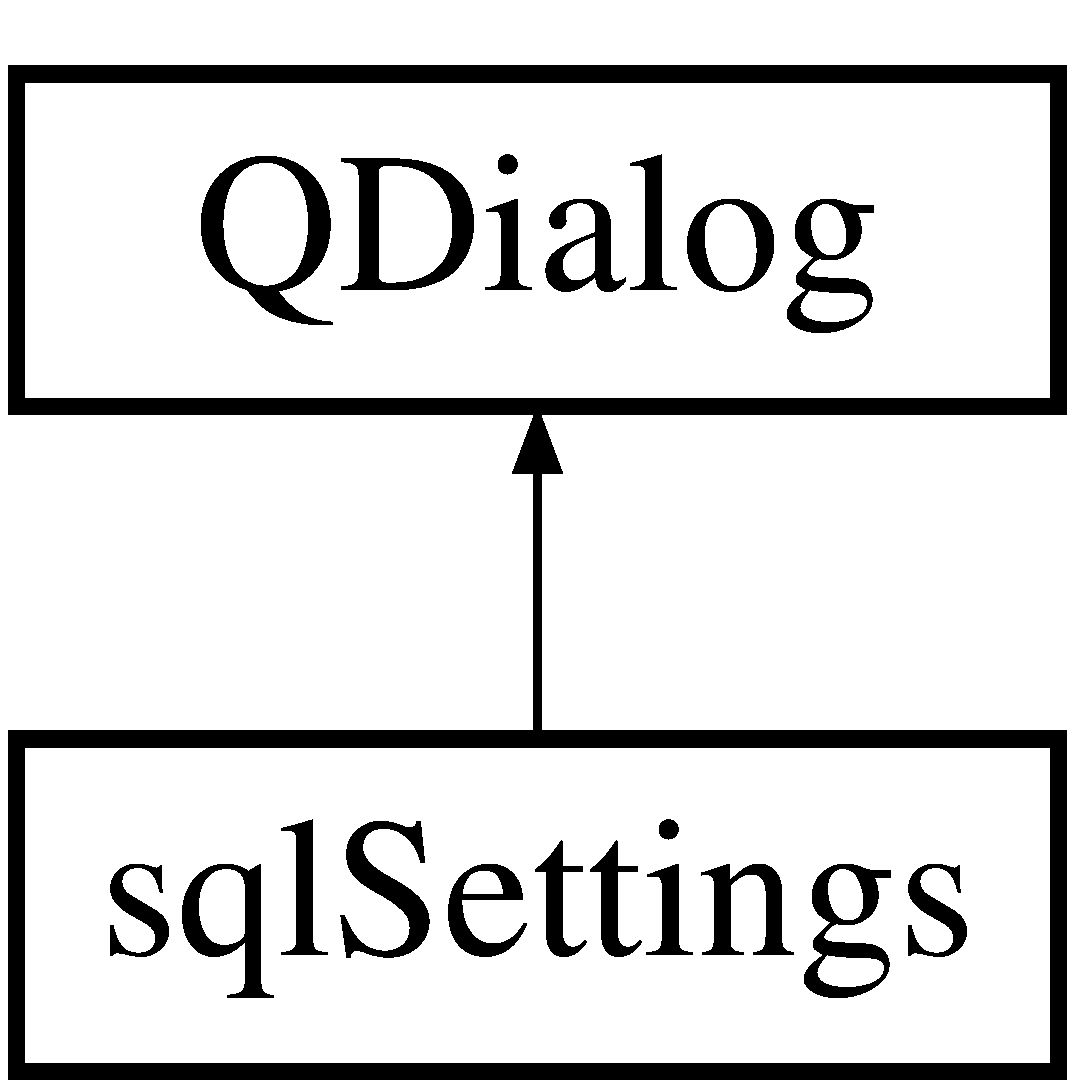
\includegraphics[height=2.000000cm]{classsql_settings}
\end{center}
\end{figure}
\subsection*{Public Member Functions}
\begin{DoxyCompactItemize}
\item 
\hypertarget{classsql_settings_afc3f1c17e3411591884f39eb18cc422d}{}\label{classsql_settings_afc3f1c17e3411591884f39eb18cc422d} 
{\bfseries sql\+Settings} (Q\+Widget $\ast$parent=0)
\item 
\hypertarget{classsql_settings_a4cb786c02dcea08898d80b2b81d7968d}{}\label{classsql_settings_a4cb786c02dcea08898d80b2b81d7968d} 
bool {\bfseries Chek\+\_\+ip} (Q\+String ip)
\item 
\hypertarget{classsql_settings_acb4db062330c05fec1054ad55f5a9ea9}{}\label{classsql_settings_acb4db062330c05fec1054ad55f5a9ea9} 
void {\bfseries set\+Begin\+Seting} ()
\end{DoxyCompactItemize}
\subsection*{Public Attributes}
\begin{DoxyCompactItemize}
\item 
\hypertarget{classsql_settings_aaf949d34fdb177a030283c3ec99833b0}{}\label{classsql_settings_aaf949d34fdb177a030283c3ec99833b0} 
\hyperlink{class_s_q_l_c_o_n}{S\+Q\+L\+C\+ON} $\ast$ {\bfseries ptr}
\end{DoxyCompactItemize}


The documentation for this class was generated from the following files\+:\begin{DoxyCompactItemize}
\item 
sqlsettings.\+h\item 
sqlsettings.\+cpp\end{DoxyCompactItemize}

%--- End generated contents ---

% Index
\backmatter
\newpage
\phantomsection
\clearemptydoublepage
\addcontentsline{toc}{chapter}{Index}
\printindex

\end{document}
